Viscosity is a property of fluids (liquids and gases) which determines how much resistance is experienced by an object trying to move through the fluid. In this experiment we will use Stoke's Law and the concept of terminal velocity to determine the viscosity of glycerin.

\section*{Objective}

   Use Stoke's Law to derive an equation relating the viscosity $\eta$ of a fluid to the time $t$ it takes for a sphere to fall a distance $d$ through it.

\section*{Experimental Setup}

   The equipment consists of a long glass cylinder filled with glycerin. A graduated scale is attached to the cylinder which allows us to measure distances along the cylinder.
   
   Small metallic spheres are dropped from the top of the cylinder. The viscosity of the glycerin produces a drag force that will eventually result in terminal velocity being achieved by the falling sphere. The terminal velocity is calculated by measuring the time $t$ it takes the sphere to fall through a distance $d$ inside the fluid.

   \tikzsetnextfilename{setup_theory}

{           % We use braces to confine the namespace and avoid conflict since we import diag/setup_defs in setup_experiment as well
   % The definitions used by the two setup diagrams

% Define the height of the cylinder. We define it outside because this is also used by the flask
\def\Ch{5}
\def\Chw{0.5}

% Define the cylinder as an embeddable drawing
\newdrawing{\cylinder}{

      \def\hw{\Chw}      % Half width of cylinder
      \def\h{\Ch}         % Height of Cylinder
      \def\uw{0.2}      % Width of top-edge of cylinder

      \draw                         % Cylinder
         (-\hw,0) -- (-\hw,\h)
         (\hw,0) -- (\hw,\h)
         (-\hw,0) -- (\hw,0)

         (-\hw,\h) -- (-\hw-\uw,\h)
         (\hw,\h) -- (\hw + \uw,\h)
      ;
}

% Define the conical flask
\newdrawing{\flask}{

   \def\chw{0.1}       % Half-width of lower column
   \def\ch{0.75}           % Height of lower column

   \def\thw{0.8}        % Half-width of the top of the slanting bit
   \def\th{0.5}         % Height of the top of the slanting bit

   \coordinate (ol) at (-\chw, 0);
   \coordinate (or) at (\chw, 0);


   % We will place the origin horizontally center and vertically where the slanting part meets the lower column
   \draw
      (ol) -- (-\chw, -\ch)
      (or) -- (\chw, -\ch)

      (ol) -- (-\thw, \th)
      (or) -- (\thw, \th)
   ;
}


   \begin{center}
      \begin{tikzpicture}

         % The common drawing instructions for the two setup diagrams

\cylinder
\flask[yshift=\Ch-0.1]    % Place flask with its anchor (origin) just below the top of the cylinder

\def\ar{1}                % Draw the miniscus of the glycerin
% To draw an arc with center (0, \Ch), radius \ar and starting and ending angles -60 to -120 we use the 'shift' option.
% The arc command uses a starting point and then angles and radius and NOT the center
% To overcome this we define the starting point as the center shifted to the starting point using polar coordinates. The ability to shift using polar coordinates is very useful here.
% So [shift=(-60:\ar)] applied to the coordinates of the center gives the starting position.
% The second part containing the start and end angles and the radius of the arc are straight-forward
\draw ([shift=(-60:\ar)] 0,\Ch) arc (-60:-120:\ar);

\def\sr{0.05}
\draw (0,2.5) circle [radius=\sr];       % The falling sphere
\draw [->] (0,2.5-\sr) -- (0,2.2);


      \end{tikzpicture}
   \end{center}
}


\section*{Free-Body Diagram}

   A sphere falling through a fluid experiences three forces: its weight $W$, an upward buoyant force $F_B$ (Archimedes' Principle) and the drag force $F_D$ (Stoke's Law) also in the upward direction since it opposes the downward motion of the sphere.

   \tikzsetnextfilename{freebody}      % We set the filename which will be used for the pdf created by the externalize library. The prefix is still applicable so build/freebody.pdf will be created
\begin{center}
   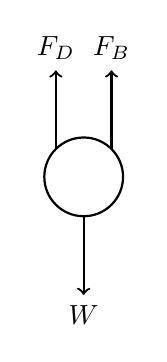
\begin{tikzpicture}

      \def\r{0.5}
      \def\h{1}

      \draw 
         (0,0) [thick] circle [radius=\r];

      \draw [thick] (0, -\r) [->] -- ++ (0,-\h) node [below] {$W$};

      \draw [thick] (45:\r) [->] -- ++ (0, \h) node [above] {$F_B$};

      \draw [thick] (135:\r) [->] -- ++ (0, \h) node [above] {$F_D$}; 

   \end{tikzpicture}
\end{center}


\section*{Derivation}

   The three forces acting on the falling sphere are given by
   \beqc \label{three_forces}
      W = m g\\
      F_B = \sigma \, V g\\
      F_D = 6 \pi \, \eta \, r v\\
   \eeqc
   where $\sigma$ is the density of the fluid and the last equation is a statement of Stoke's Law which describes the drag force acting on a sphere of radius $r$ as it moves with velocity $v$ through a fluid with viscosity $\eta$.

   The first two forces remain constant but the drag force increases in magnitude as the sphere speeds up since it is directly proportional to the velocity $v$. Initially, when the velocity of the sphere is low, the drag force is low as well and therefore the net downward force and acceleration are large. This causes the velocity to increase. As the velocity increases the drag force increases and in turn the net downward force and acceleration decrease. The velocity keeps increasing but at a slower rate. Eventually the drag force increases until it exactly balances the other two forces. The net downward force and acceleration become zero and the velocity becomes constant. This is known as the terminal velocity $v_T$.

   Therefore, by definition, when the terminal velocity is achieved the net force on the sphere is zero, the three forces balance each other out. Looking at the free-body diagram this means
   \beq
      W = F_B + F_D
   \eeq
   \def\stokes{6 \pi \, \eta \, r v_T}

   Substituting \eqref{three_forces}
   \beqn
      \imply m g = \sigma \, V g + \stokes 
   \eeqn

   The mass of the sphere $m$ can be expressed in terms of the density $\rho$ of the sphere as $m = \rho V$.
   \beqcn
      \imply \rho V g = \sigma \, V g + \stokes\\
      \imply \stokes = \rho V g - \sigma V g\\
      \imply \stokes = (\rho - \sigma) V g
   \eeqcn

   The volume of a sphere is given by $V = \frac{4}{3} \pi r^3$. If the sphere (after attaining terminal velocity) falls through a distance $d$ in time $t$ the terminal velocity can be calculated using $v_T = \frac{d}{t}$. Substituting these in
   \beqcn
      \imply 6 \pi \, \eta \, r \frac{d}{t} = (\rho - \sigma) \frac{4}{3} \pi r^3 g\\
      \imply 3 \, \eta \, \frac{d}{t} = \frac{2}{3} (\rho - \sigma) g \, r^2\\
   \eeqcn

   Since our aim is to calculate the viscosity of the fluid we make $\eta$ the subject of the equation giving us

   \beq
      \eta = \frac{2}{9} \frac{(\rho - \sigma) g \, r^2 t}{d}
   \eeq

   Thus we end up with an equation that relates the viscosity of a fluid to the radius of the sphere falling through it and the time it takes for it to fall through a certain distance. This equation governs the working of a \textbf{viscometer} a device where falling spheres are used to measure the viscosity of a fluid.
